 
% ME3001   
% Tristan Hill - Spring 2024 
% Finding Roots of Non-Linear Functions 
% Mechanical Design through Optimization


% Document setting
\documentclass[11pt]{article}
\usepackage[margin=1in]{geometry}
\usepackage[pdftex]{graphicx}
\usepackage{multirow}
\usepackage{setspace}
\usepackage{hyperref}
\usepackage{color,soul}
\usepackage{fancyvrb}
\usepackage{framed}
\usepackage{wasysym}
\usepackage{multicol}

\pagestyle{plain}
\setlength\parindent{0pt}


% assignment number 
\newcommand{\NUM}{2} 
\newcommand{\HSPC}{42mm} 
\newcommand{\HHSPC}{33mm} 
\newcommand{\VSpaceSize}{2mm} 
\newcommand{\HSpaceSize}{2mm} 

\definecolor{mygray}{rgb}{.6, .6, .6}

% [153,50,204] - dark orchid
\definecolor{mypurple}{rgb}{0.6,0.1961,0.8}
%[139,69,19] - saddle brown
\definecolor{mybrown}{rgb}{0.5451,0.2706,0.0745}


\begin{document}

	\textbf{\LARGE ME3001 - Spring 2024} \\\\
	\textbf{\LARGE Weekly Activity \NUM:  Roots of Non-Linear Equations}\\\\
	\textbf{\LARGE Mechanical Design through Optimization} \\
	
	\begin{description}
        \vspace{5mm}
    \item [\textbf{ \Large Overview}] \textbf{ \Large :}\\
	
				As an engineer you are asked to design a structure. The geometry of this structures is simple but certain properties are critical. Also you want to spend as little as possible on materials.
					
				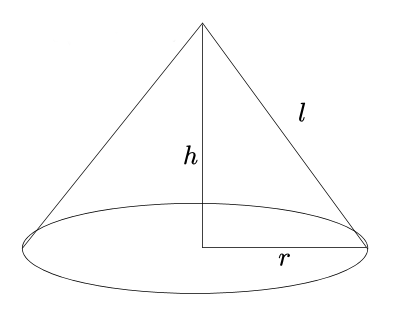
\includegraphics[scale=.35]{lecture3_fig1.png}\\
					
				You are required to design is a cone with a surface area of exactly $25 m^2$ to a tolerance of 0.1 $m^2$ and a height of exactly $1 m$. Your goal is to find the radius in meters.\\
    \item [\textbf{ \large Assignment}] \textbf{ \Large :}\\

  \begin{enumerate}

    \item 

Solve the mechanical design problem decribed above using a method of your choice in MATLAB. The goal is to find a value of r such that the cone has the specified surface value.

  \end{enumerate}

  \item [\textbf{ \large Deliverables}] \textbf{ \Large :}\\
    \begin{itemize} 
   
      \item MATLAB Code:
Write a MATLAB program use a method of your choice to solve the given problem. The solution strategy should be clearly defined and documented. Submit the .m file(s) used and document any example code that you used or learned from during the exercise.

      \item Results:
Submit a brief summary of the problem statement and present the results from the solution code. The results can be typed in the program comments or typed in the assignment text box.

    \end{itemize}
  \end{description}
 
\end{document}



